\documentclass[letterpaper,twocolumn,amsmath,amssymb,pre]{revtex4-1}

\usepackage{graphicx}% Include figure files
\usepackage{color}

\newcommand{\red}[1]{{\bf \color{red} #1}}
\newcommand{\blue}[1]{{\bf \color{blue} #1}}
\newcommand{\green}[1]{{\bf \color{green} #1}}

\newcommand{\fixme}[1]{\red{[#1]}}
\newcommand{\davidsays}[1]{{\color{red} [\green{David:} \emph{#1}]}}

\newcommand\micron{\ensuremath{\mu\text{m}}}

\begin{document}
\title{Robustness of MinD oscillation in \emph{Escherichia coli} with
  diverse cell shapes}

\author{Jeff B. Schulte}
\affiliation{Department of Physics, Oregon State University}
\author{Rene WHAT. Zeto}
\affiliation{Department of Physics, Oregon State University}
\author{David Roundy}
\affiliation{Department of Physics, Oregon State University}

\begin{abstract}
  The dynamics of the Min-protein system help Escherichia coli
  bacteria regulate the process of cell division by identifying the
  center of the cell.  We model the Min-protein system in bacteria
  that have been forced into unusual flattened shapes, as have
  recently been experimentally observed.  We find that although the
  presence of Min oscillations is robust in a wide variety of cellular
  configurations, the location of the peaks is strongly affected by
  the cellular shape.  In some cases no periodic oscillations are
  observed.  In particular, we find that cellular shapes observed
  experimentally to present irregular oscillations do so in the
  theoretical model, consistently \fixme{or inconsistently?} with
  experiment.  \fixme{In agreement with previous theoretical and
    experimental results, we observe ``rotating'' behavior in certain
    shapes having three corners.}
\end{abstract}

\maketitle

\section{Introduction}
It is vital that during the process of bacterial cell division a cell
avoid minicelling, or splitting into daughter cells with lopsided
volumes.  During this process a long FtsZ polymer chain develops on
the cell wall in the center region of the cell that dictates the plane
of division~\cite{adams2009bacterial,
  lutkenhaus2007assembly}. Previous experimental studies have shown
that the MinC protein, known to inhibit the FtZ
polymer\cite{shen2010examination}, exhibits a pole to pole oscillatory
behavoir in conjunction with the MinD and MinE proteins, while the
oscillating MinE tends to be more localized in the center of the
cell~\cite{hu1999topological, fu2001mine, shapiro2009and, yu1999ftsz,
  raskin1999rapid}. The MinC protein will then have a higher time
averaged concentration in the cell poles as opposed to the center
region of the cell, aiding in prohibiting the FtZ from developing in
the wrong region.

It is vital for the mechanism by which the cell accurately divides to
be robust and indeed it has been shown to
be\cite{touhami2006temperature}.  Studies have shown that the
oscillations can effectively find poles in abberent cell
shapes~\cite{corbin2002exploring} \cite{juarez2010changes}.  Varma et
al. have studied three pronged connected tube shapes, both
experimentally and in simulation\cite{varma2008min} and have shown
that even in these oscillations develop in regular patterns. However,
Mannik et al. have shown that there are limits to this
robustness. Forcing cells into flattened, irregular cell shapes
adversly effects the Min system's ability to maintain their regular
oscillatory behavior \fixme{this link doesn't work =
  cite{mannik2012robustness}} \cite{mannik2010bacteria}
\cite{mannik2009bacterial}.  We follow the experimental work of Mannik
et and use Huang's mean field differential equation reaction model to
explore the model's ability to find regular oscillatory behavoir in a
series of abberent shapes.  \davidsays{This paragraph could use some
  work, and should reference Mannik early, and emphasize his research.
  First paragraph sets the stage for why our work is important by
  introducing the MinD system.  Second paragraph should explain why we
  are studying the Min system in funny cell shapes.}

A significant amount of work has been done to develop protein reaction
and diffusion models that exhibit accurate macroscopic dynamics of the
MinD protein system. Early models involved free proteins that affect
eachothers' rates of diffusion and membrane attachement but do not
combine into compound states~\cite{meinhardt2001pattern}.  In 2003
Huang improved upon this work with a simple model based on MinD-MinE
combination, ATPase hydrolysis, and MinD membrane attechent that when
simulated exhibits accurate MinD oscillations in cylindrical
cells~\cite{huang2003dynamic}. In this model cytoplasmic MinD is more
likely to attach to the membrane when MinD is already clustered there
(following observed non-linear attachement of minD on the cell
membrane), and is stationary once attached.  A number of studies have
used an approach similar in that they do not rely on the ability of
MinD to move along the walls and
cluster~\cite{kruse2007experimentalist, meinhardt2001pattern,
  drew2005polymerization, fange2006noise, kerr2006division}, while
studies have been made as well of models which rely on MinD mobility
and attraction on the cell membrane~\cite{kruse2002dynamic,
  howard2005cellular}.  Variations of the Huang 2003 model that
stochasticly account for variations of molecular interaction
\cite{fange2006noise} and as well monte-carlo simulations that
implement stochastic version of Huang's mean filed reaction rates
confirm the major results obtained by Huang's model and more
successfully predict experimentally observed oscillations in round
cell phenotypes~\cite{drew2005polymerization, fange2006noise,
  huang2004min}. Biochemical models of broader scope have also been
used to study the MinD system and show consistent
results.\cite{arjunan2010new}.  However, in general the results of the
stochastic and monte-carlo simulations are similar to those given by
Huang's mean field results.

Previous studies have been made of the Min system's associtation with
the cell membrane
\cite{hsieh2010direct}\cite{mileykovskaya2003effects}.  Studies have
shown as well that MinD binds preferentially to regions enriched with
cadiolipin, an anionic phospholipid that collects on regions of high
negative curvature. This mechanism has been incorporated into other
models.\cite{drew2005polymerization,cytrynbaum2007multistranded,renner2012mind,renner2012mind}
However, this mechanism of combined clustering, phospholipids and MinD
has not been observed in real cells. \cite{halatek2012highly}

\begin{figure}
  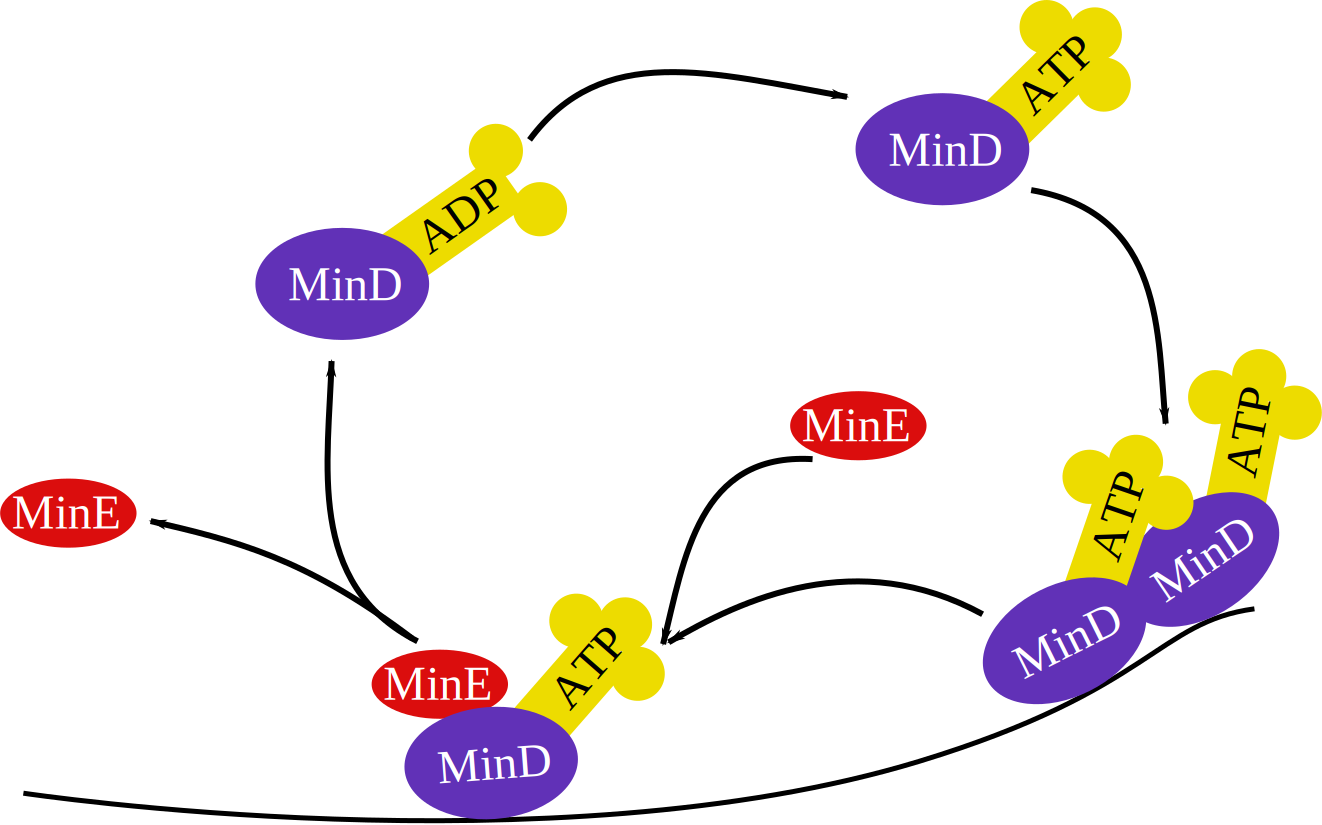
\includegraphics[width=\columnwidth]{reactions}
  \caption{Reactions included in the model of Huang \emph{et
      al.}~\cite{huang2003dynamic}.}\label{fig:reactions}
\end{figure}

\section{Model and Methods}
We implement the model of Huang \emph{et al.}  for the behavior of the
MinD and MinE proteins inside the cell~\cite{huang2003dynamic}.  This
model is defined by a set of five reaction-diffusion equations:
\begin{align}
  \frac{\partial n_{?}}{\partial t} &= \text{\davidsays{Actual differential equations here.}}
\end{align}
These equations define the rates of diffusion and reaction shown in
Figure~\ref{fig:reactions}.  \davidsays{Add more text here, describing
  the system and the reactants.  In particular, we want to state that
  MinD:ADP binds ATP (or is hydrolyzed?... check!) to form MinD:ATP,
  which then gets stuck to the cell membrane, which is more likely
  when there is already MinD:ATP bound to the membrane.  The MinE then
  binds to the membrane-bound MinD:ATP.  Finally the whole complex can
  fall off the membrane, at which stage you end up with MinD:ADP and
  are ready to start over.  This is also where we define our
  terminology for the volume and surface densities.}


The reaction shown in Figure~\ref{fig:reactions} is cyclical so we can
begin our observations at any stage in the cycle (which is presented
for the natural cell shape in Fig.~\ref{image-p} below).  We consider
first MinD:ATP floating freely in the cytoplasm.  The protein will not
react with any other floating protein, and it will not spontenously
shift back into the MinD:ADP stage of the cycle.  It will diffuse
until it attaches to a cell membrane.  This is will happen most
rapidly in regions of high curvature, where diffusion is more likely
to lead to an encounter with a wall.  This effect is made more
pronounced by the MinD:ATP tendency to attract and cluster on the
membrane, as reflected in Equation~\ref{eq:d-on-wall}, which shows
that when adjacent to the membrane, the rate of binding to the
membrane is porportional to the amount of MinD already bound to the
wall.  Initially, then, there is a strong tendency of MinD to cluster
on the polar regions of the cell, where the curvature is highest.

We next see the formation of MinE `rings' on the membranes of the
polar caps.  As the freely diffusing MinE enters the cap portion it
begins to encounter concentrated membrane bound MinD.  The MinE binds
to this MinD and remians for a time on the walls in compound form.
When it is released, it can diffuse naturally outward or inward
towards the cell.  If it diffuses inward, there is less cross
sectional wall for it to bump into and also less concentrated MinD:ATP
to react with.  If it diffuses outward, the curvature of the cell wall
cuases there to be a greater chance that it will encounter the cell
membrane (for the same reason outlined for the MinD:ATP above) and if
there is MinD:ATP bound there, there is a chance that it will bind to
that protein and react again.  If it does diffuse in this directin, it
will likely react with MinD:ATP before getting very far into the
encap.  Thus after dettaching from the membrane at the edge of the
MinD:ATP encap cluster, the MinE is most likely to travel a small
distance further into the polar region and then attach and react again
with MinD:ATP protein there.  This process results in the observed
qualitative 'encroaching MinE ring' behavoir that releases MinD:ADP
back into the cytoplasm.  This MinD:ADP will diffuse for a time before
spontanosly uindergowing hydrolysis \fixme{is this right?} and
reaching the MinD:ATP state that can bind to the membrane again.
There is a strong chance that it has by this time diffused out of the
polar region and is on its way to the opposite polar region of the
cell.  If it hasn't then it will reattach to the MinD:ATP on the cell
wall deeper into the endcap and will eventually be converged upon by
the MinE ring, only to be released again in MinD:ADP form.

Overall this process results in an extremely robust oscillatory
behavoir of polar selection and oscillation in a wide variety of cell
shapes.



 A 3d grid is constructed in cartesian
coordinates with a grid spacing of .05\micron. We define our cell
shapes and solve the reaction-diffusion equations numerically to
observe the time evolution of the MinD and MinE concentrations inside
the cell.

We start our cells with the MinD and MinE concentrations that are
reported as wild type concentrations by Huang et al . We as well use the same reaction
diffusion constants and and reaction rates,
\begin{gather*} %format better
  \mathcal{D}_D = \mathcal{D}_{E}  = 2.5 \micron^2/\text{sec}, \\
  \sigma_D^{\textrm{ADP $\rightarrow$ ATP}}  = 1/\textrm{sec},  \sigma_D = 0.025 \micron /\textrm{sec}, \\
  \sigma_{dD}  = 0.0015 \micron^3/ \textrm{sec}, \\
  \sigma_{de}  = 0.7/\textrm{sec}, \sigma_E = 0.093 \micron^3 /\textrm{sec}.
\end{gather*}

\section{Cell shapes}

In order to address the limits at which the stability of the
oscillations of the Min system break down, as observed by Mannik
\emph{et al.}~\cite{mannik2012robustness}, we model the Min system in
a variety of cell shapes.  We begin with natural pill-shaped cells,
and the proceed to examine a number of flattened pancake-like shapes,
which reflect the experiment of Mannik \emph{et al.}, in which
bacteria were confined within a thin slit~\cite{mannik2012robustness}.
Our pill shapes differ from those of Huang \emph{et al.} in that they
are cylinders with hemisphere endcaps instead of pure cylindridrical
shapes. \davidsays{Double-check the Huang paper on their shapes.}  Our
cylinderidrical radius is $0.50\micron$ and the lengths of our cells
(measured between the tips of the endcaps) are $5\micron$, $4\micron$, $3\micron$,
and $2.5\micron$.

With our flattened cell shapes we mean to study cells that are
parrallel to those lodged into crevices by Mannik so we give them
height of $0.25\micron$ \cite{mannik2012robustness}.  Viewed from the top
down the cells will have the shapes described below and viewed from
the side they have at their edges a semicircular protrusion (one may
imagine the edges of a pancake).

Our first group of (three) flattened cell shapes are triangular.  One
of them is equilateral, one has a 3-4-5 right angle shape, and the
last is iscoscolese.

Our second group of (four) flattened cells are our own creations,
designed to investigate different patterns of protein oscillation
behavoir.

The cell shapes and the sections that we split them into in our data
analysis are shown in Figure \fixme{We need a big figure with all of this!!}.

Kubitschek has shown in multiple experiments that at the time of cell
division cells have a volume that is within a range of roughly
$1\micron^3$ to $2\micron^3$~\cite{kubitschek1990cell,
  kubitschek1968linear}.  We follow Huang's
simulations\cite{huang2003dynamic} and Mannik's experiments
\fixme{this link doesn't work = cite{mannik2012robustness}} and model
cells that are slightly larger than this range.  Amoung our flattened
cells the two dimensional length scales are tuned so that every total
cell volume is very close to $3\micron^3$.  \fixme{should we just
  leave it to the reader to figure out for themselves what our pill
  shape volumes are?}


To interpret the results, we generated several different plot views of
the printed simulation data. These plots included a time averaged view
of the protein densities in the cell; a plot tracking the location of
protein concentrations that were global maxima in space and local maxima in
time; and an animated view that showed the actual dispersion of
protein concentrations in the cell over time.
\section{Specific Results}

\subsection{Pill Shape}

\begin{figure*}
  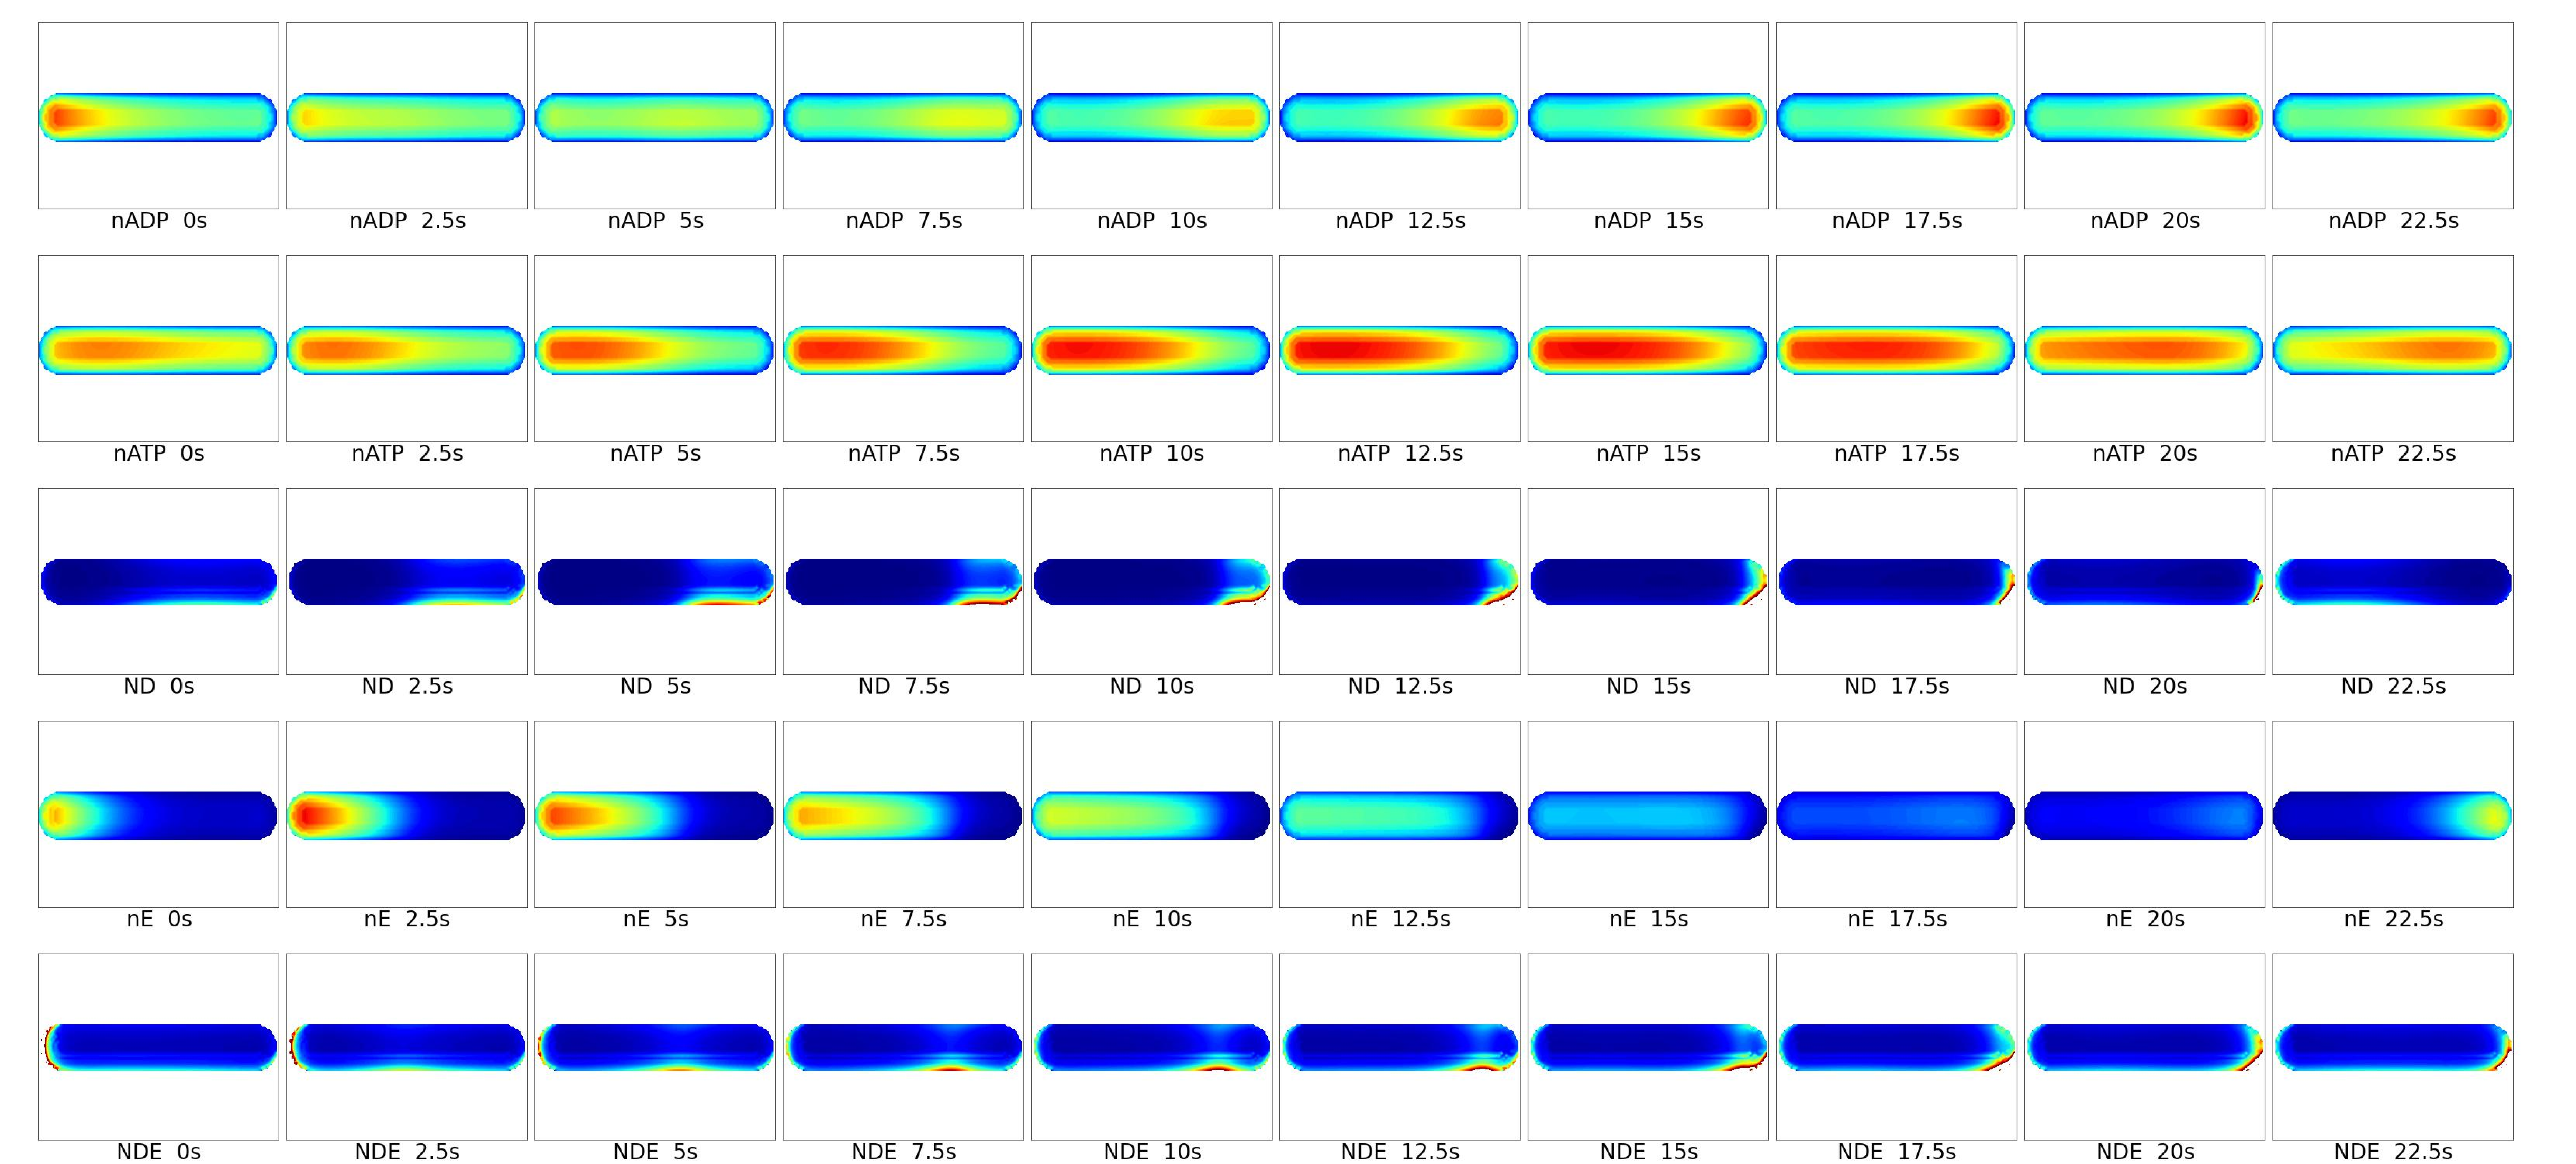
\includegraphics[width=\textwidth]{../data/shape-p/plots/image-plot--p-400-50-0-0-1500.pdf}
  \caption{Frames from an animation showing a series of contour plots
    of the concentration of proteins in different stages over time.
    The density of proteins are integrated along the axis normal to
    the page. The frames occur 2.5 seconds apart. \fixme{this looks
      assymetric! That's a big problem.} \davidsays{I like this plot,
      but would rather see it improved in a few ways.  I noticed the
      implementation combines together bitmaps.  Nicer would be to use
      subplots within matplotlib, so we output the plot directly as a
      pdf.  Then we could also arrange things so there is much less
      vertical white space.  It'd be nicer to have labels at the left
      and a time axis at the bottom, with no labels by each image.  I
      know this will take a while, so it's not yet a high priority.}}
  \label{image-p}
\end{figure*}

We begin with the naturally occuring pill shape.  We peice this shape
together as two hemispherical endcaps attached on either end of a
cylinder.  This shape follows the early simulations of Huang \emph{et
  al.} but differs in that we have added the end caps for a more
natural shape, expecting similar results.  We test cells of radius
$.5\micron$ and of lengths $2\micron$, $3\micron$, and $5\micron$
between both tips of the end caps. In all these models we observe
quick establishement (within a few periods) of extremely regular
oscillatory behavoir that lasts indefinitely, with periods that
closely agree with the results of Huang \emph{et al.}
Table~\ref{tab:pill-periods} shows the periods of oscillations
at different cell lengths.

\begin{table}
  \begin{tabular}{|r|c|c|c|l|}
    \hline
    Length($\mu$) & 2.50 & 3.00 & 4.00 & 5.00\\
    \hline
    Period(sec) & sim & 33 & 38 & 48 \\ \cline{2-2}
    \hline
  \end{tabular}
  \caption{Period According to Pill Length}\label{tab:pill-period}
\end{table}

This simple model is a good starting point for observing in detail the
dynamic interaction between the different stages of protein that lead
to their qualitatively distinct behavoir. Figure \ref{image-p} shows
the process in a series of frames taken from simulation animations.
Each frame is 2.5 seconds ahead of the last.

Consider Figure \ref{image-p}.  In the beginning, the cytoplasmic
nATP is roughly evenly distributed throughout the cell.  There is nADP
concentrated in the left pole and it will transform into nATP.  At 2.5
seconds we see membrane bound MinD:ATP form on the right side of the
cell.  It avoids the left side because there is a concentration of
cytoplasmic MinE on the left side and compared to the right side,
which is empty of MinE, MinD:ATP attaching to the wall on the left has
no time to collect and cluster before reacting.  One can see how as
the MinE spreads out rightward, the the clustered membrane bound
MinD:ATP stays just at the edge of it, always to the right.  Where the
two meet there is at every time step a spike in membrane bound
MinD-MinE:ATP, resulting from the MinE reaction with the MinD on the
wall.  One can see from roughly 5 seconds to 17.5 seconds the
cytoplasmic MinE chases in a way the MinD towards the right, reacting
with it as it clusters on the wall.  Upon reaching the right side, the
MinD is in a way trapped, and the MinE now concentrated in that pole
will react until the MinD has diffused back towards the other side and
there is no more membrane bound MinD:ATP to react with.  The cycle
then begins again.



\begin{figure}
  %%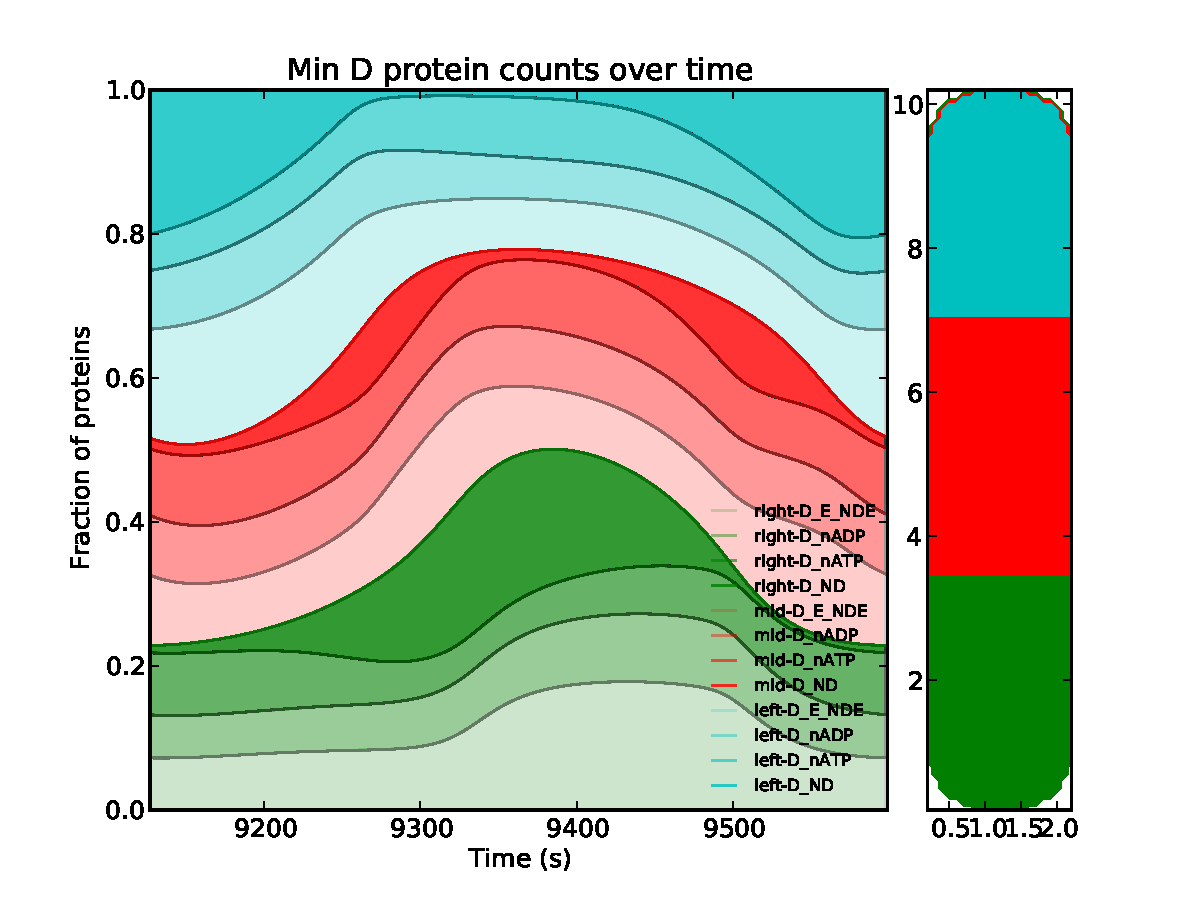
\includegraphics[width=\columnwidth]{../data/shape-p/plots/box-plot_D--p-400-50-0-0-1500}
  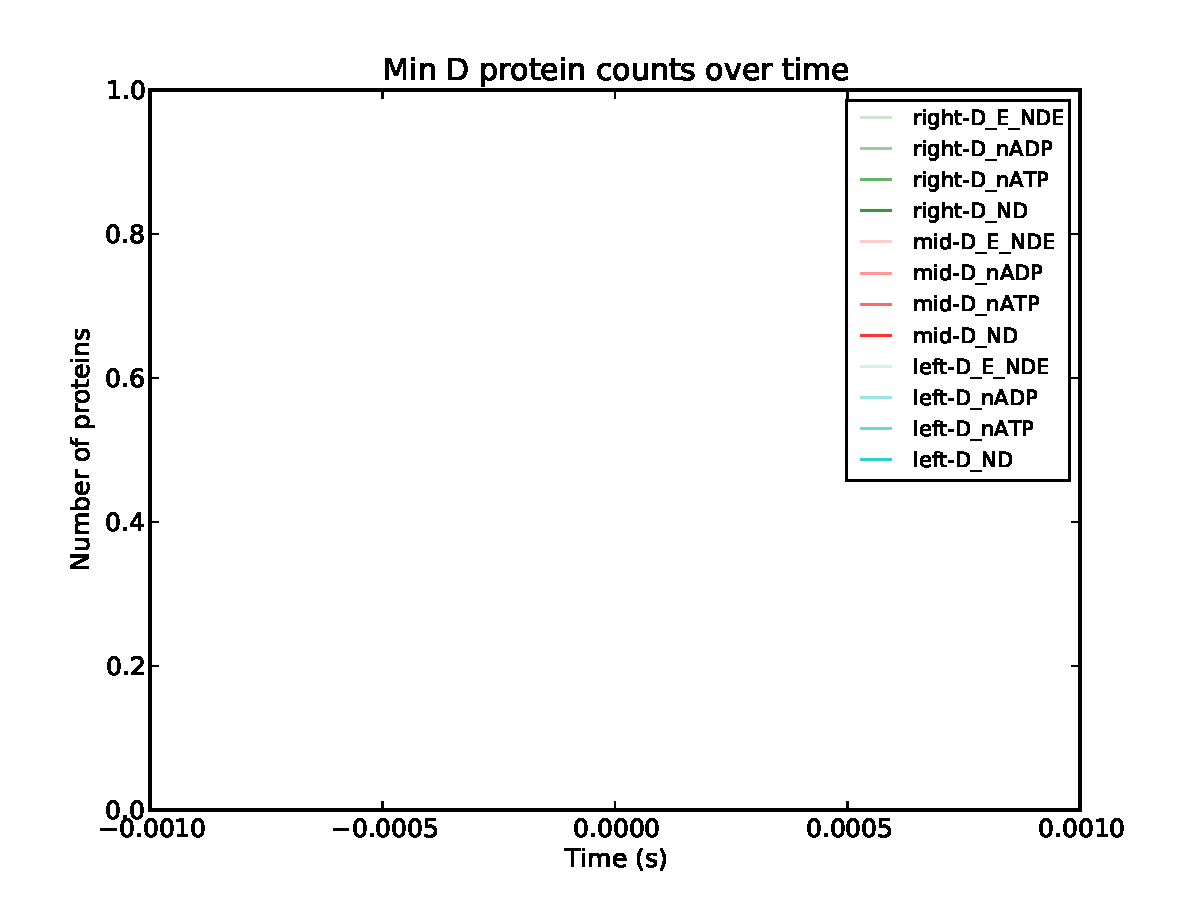
\includegraphics[width=\columnwidth]{../data/shape-p/plots/box-plot_D--p-200-50-0-0-1500}
  \caption{Total protein fluctuation in the right, middle, and left
    parts of a 5$\micron$ by 1$\micron$ pill shaped cell (above) and a
    3$\micron$ by 1$\micron$ pill shaped cell (below).  The vertical axis shows
    stacked the total number of proteins that are of four different
    compound stages and in the right section of the cell (bottom four
    colors), in the middle of the cell (middle four colors) and in the
    left section of the cell (top four colors). The different forms of
    protein changes while the total number of MinD protein in the cell
    remains constant, shown by the fact that the very top line is
    horizontal.}
  \label{box-p}
\end{figure}

Figure \ref{box-p} is a plot of the total fraction of
MinD found in each stage of the cycle in each of three sections of the
cell (we have split the pill into two polar sections and one center
section) over time.  One complete oscillation period is shown, in
which one of the poles begins and ends at a maximum density
concentration and the other a minimum density concentration.  Looking
at the evolution of the latter, we see an initial high concentration
of cytoplasmic MinD:ATP, as the this protein diffuses into the polar
region, followed by a dip in this and large spike in membrane bound
MinD:ATP, as the protein clusters onto the polar cell wall, followed
by a spike in the memebrane bound MinE:MinD:ATP stage of protein,
together with a slight rise in cytoplasmic MinD:ADP as the MinD
dettaches from the wall.

results for pill shaped cell of length
$5\mu$ and radius $.5\mu$.  The plot shows both the transerence
between different stages of protein compound and movement within the
cell.  Starting at the beginning of a period, we can see that first
there is a spike on the left of MinD-ATP attached to the wall that is
accompanied by a growing number of cytoplasmic MinD-ATP and MinD-ADP
that are entering the left section, followed by a high peak in
MinD-MinE-ATP.  This peak gives way through the middle to peaks on the
right side of the cell, the first being a small bump in cytoplasmic
MinD-ATP that dissapears into a much larger spike in wall attached
MinD-ATP, which is followed by a peak in wall attached MinD-MinE-ATP.
The pattern during each period clearly shows the cycle of proteins
rections, as well as the very regular nature of the pole to pole
protein oscillations.

\fixme{our 5 length cells are labeled as 4 cells in the file labels,
  since 4 is the length of the cylinder. In the text I'll refer to the
  5 length cells (file says 4) as 5 length cells.  What huang's paper
  calls 4 length cells will be labeled by our files as 3 length cells,
  but will be refered in our text as 4 length cells}.  We can see a
clear difference in period between the $5\mu$, $4\mu$, and $2\mu$
length cells.  The oscillation periods for our $4\mu$ show excellent
agreement with the simulations of Huang et all
\cite{huang2003dynamic}.  This is to be expected since we begin our
simulations with their reported wild type concentrations of MinD and
MinE proteins. The periods for the different pill lengths are shown in
the table below.  We can see a direct correltation between size and
period, as the proteins must diffuse further in a longer cell before
they accumulate on the opposite wall.

\begin{figure}
  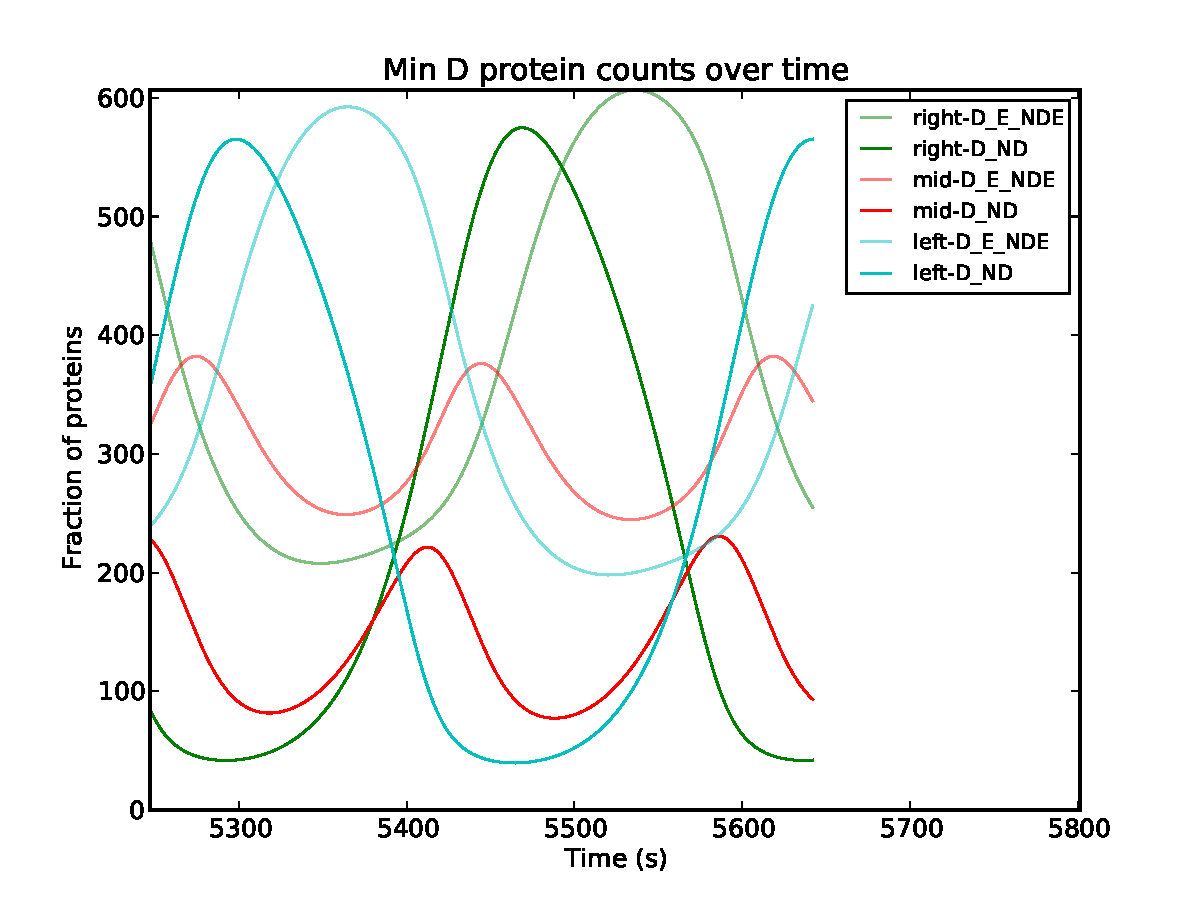
\includegraphics[width=\columnwidth]{../data/shape-p/plots/ave-plot_D--p-200-50-0-0-1500}
  \caption{Average protein density per unit area of wall for the wall
    attached stages of the protein cycle.  Shown in the right, middle,
    and left parts of a 5$\micron$ by 1$\micron$ pill shaped cell (above)
    and a 3$\micron$ by 1$\micron$ pill shaped cell (below).}
  \label{ave-per-area-plot-pill}
\end{figure}

Figure \ref{ave-per-area-plot-pill} shows the ave protein per unit
area that is wall attached in the middle, right, and left sections of
the pill shaped cell.  This is an important test of the central idea
behind the utility of the Min protein system.  The system is meant to
place Min proteins on the walls in heavier concentrations in the caps
of the cell and lower concentrations in the middle section, so that
the FtZ polymer may build up along the center walls.  We can see from
the plot of the 3$\micron$ by 1$\micron$ cell that the MinD proteins reach
concentration peaks in the caps that are higher than peaks in the
center.  \fixme{is the next part true?} Integrals of these plotted values show that the time averaged
concentrations are likewise higher in the caps than in the center.

\subsection{Triangular Shapes}
\begin{figure}
  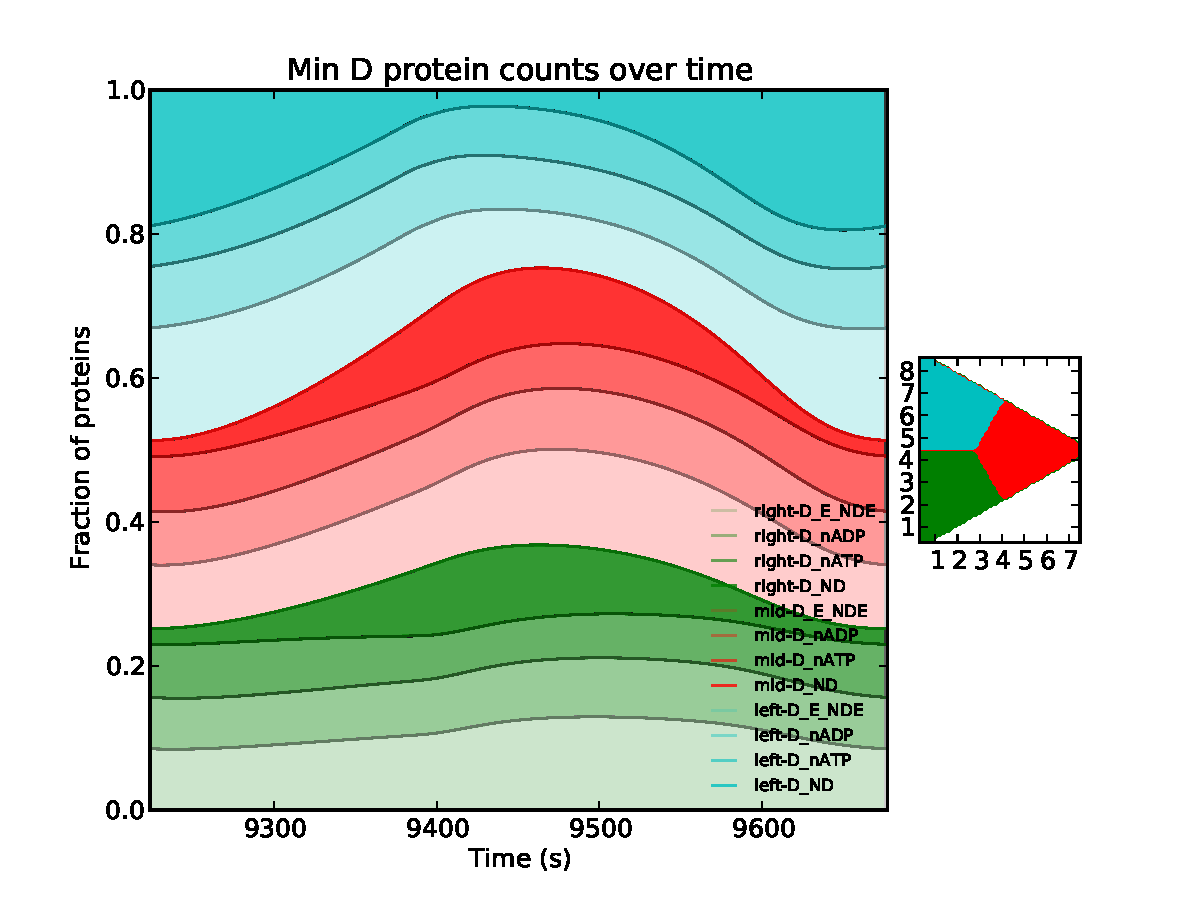
\includegraphics[width=\columnwidth]{../data/shape-triangle/plots/box-plot_D--triangle-25-400-400-400-1500}
  \includegraphics[width=\columnwidth]{../data/shape-triangle/plots/box-plot_D--triangle-25-500-300-500-1500}
  \includegraphics[width=\columnwidth]{../data/shape-triangle/plots/box-plot_D--triangle-25-600-480-360-1500}
  \caption{Total protein fluctuation in the right, middle, and left
    parts of an equilateral (top), iscoscolese (middle), and 3-4-5
    (bottom) triangle.  The vertical axis shows stacked the total
    number of proteins that are of four different compound stages and
    in the different sections of the cell.}
  \label{box-triangle}
\end{figure}

The double pole oscillation pattern, in which one pole is located in a
single corner of the triangle and the other pole is spread out between
the opposite two, can be seen in Figure \ref{box-triangle}.  The
equilateral triangle shows a spike in both the Center and Left
sections at the same time, both showing the familiar sequence of peaks
amoungst the different states of the protein seen in the poles of the
pill shaped bacteria.  A spike in the other corner, showing the common
sequence, occurs during the minima of the former two, wth a higher
concentration at the peak.  A similar pattern is seen in the
iscosolese triangular shape, where interestingly the onset of the
maxima in the single maxima corner (the Left section) builds more
quickly than it fades.  This is presumably becuase as the cytoplasmic
minD:ATP diffuses down a more accute corner, it is sourrounded by
closer cell walls than it would be in a less acute corner, so that the
it is more apt at any diffusive step to make contact and cluster on
the walls.  That particular part of the process is therefore
accelerated, driving the build up of the maxima forward.

The right triangle shows a similar pattern except that here there is
an assymetry between the two corners that maximize at roughly the same
time.  One corner is further from the single maximizing corner and it
consisitently peaks later.  The MinD simply have further to travel
before they maximize there.

For these three sizess and shapes there is not sign that the
oscillation patterns once they are set will break down.

\begin{figure}
  \includegraphics[width=\columnwidth]{../data/shape-triangle/plots/box-plot_D--triangle-25-601-601-601-1500}
  \caption{Total protein fluctuation of an equilateral triangle with
    larger dimensions (each side is roughly $6\micron$.  The vertical
    axis shows stacked the total number of proteins that are of four
    different compound stages and in the different sections of the
    cell. The time limits have been set to show the broken down
    section of the simulation.}
  \label{box-triangle}

The larger equilateral shape shows the same pattern as the smaller
version does only until fifteen periods, at which point there is a
breakdown of the oscillation pattern.  During the last three stable
periods, the single maximizing corner, the lower left section in the
figure, has a lower peak each period as the membrane bound MinD:ATP in
the other corners lag more and more before being eaten away by the
MinE.  Finally these maxima lag so much that they break down the
regular pattern.  There then occurs about five periods of semi chaotic
behavoir, until it settles back into another stable oscillation that
is similar to the original one, except that a different corner has
been chosen to be the singlular maxima (the right section in the
figure), while the other two corners maximize at the same time.  This
interesting breakdown and recovery shows both the robustness of the
double pole oscilatory tendency and the importance of required
distance of travel for the different proteins.

\end{figure}


Fifteen


\subsection{Randst shape}
\fixme{Cheat sheet for the shapes, need to put these into a big figure
  from the sections output: 96=star shape, 97=sideways sideways
  flying saucer pancake, 98=manniks squished cell, 99=an A}

\subsubsection{Randst-mannik shape}
\begin{figure}
  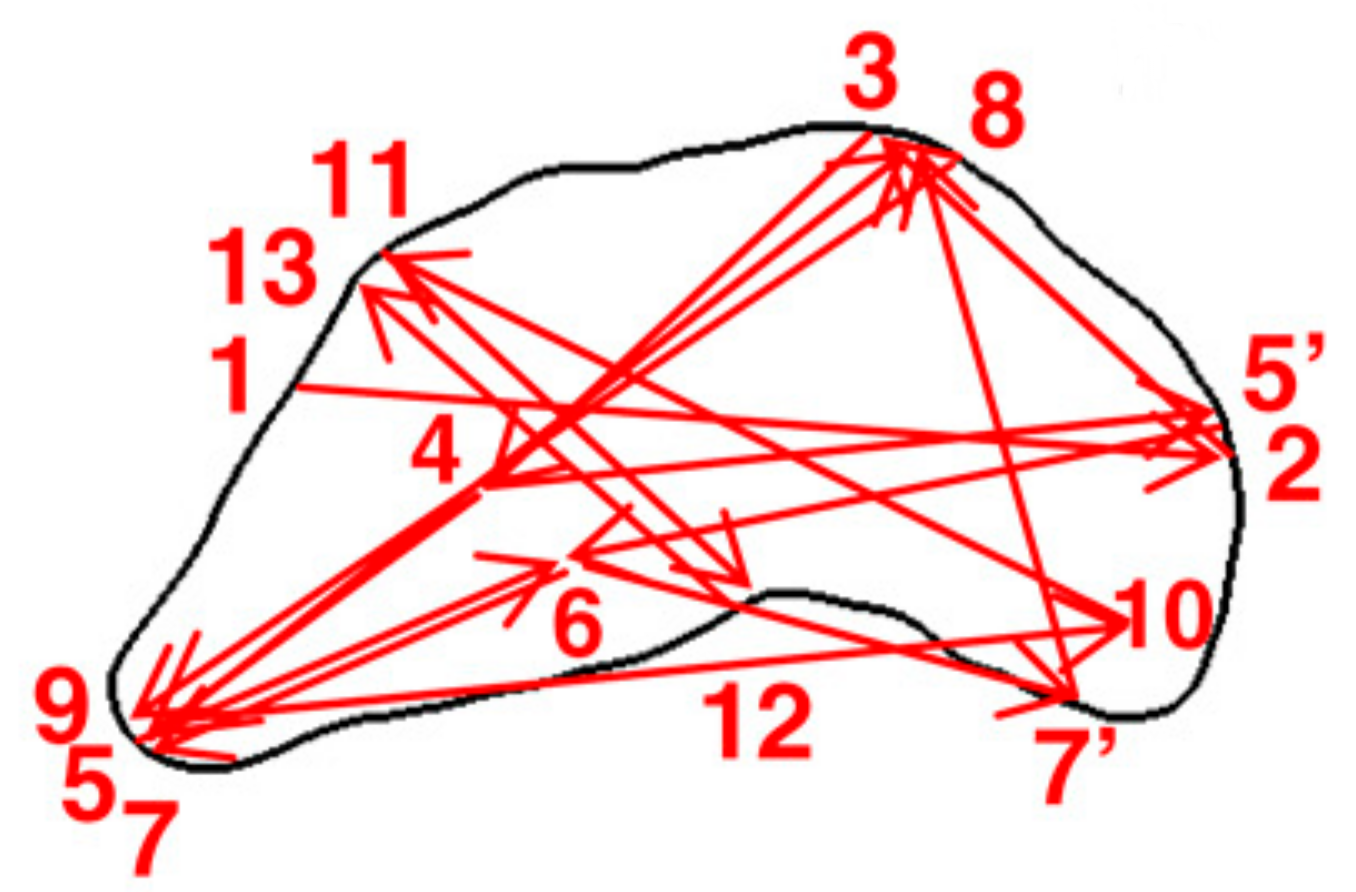
\includegraphics[width=2.8cm]{../mannik-2.png}
  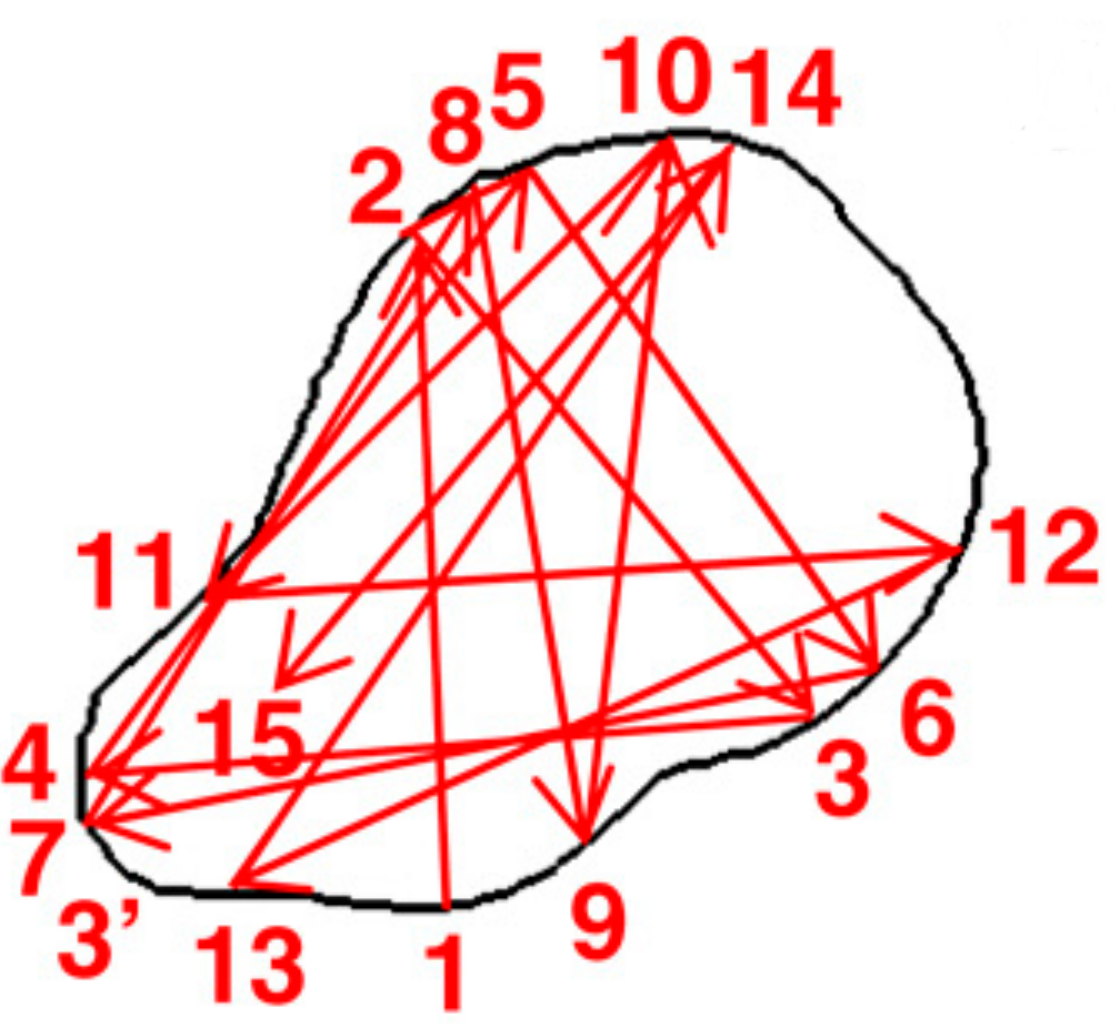
\includegraphics[width=2.8cm]{../mannik-1.png}
  \includegraphics[width=3cm]{../data/shape-randst/plots/arrow-plot-NflD-randst-25-1300-2000-9400-1500.pdf}
  \includegraphics[width=3cm]{../data/shape-randst/plots/arrow-plot-NflD-randst-25-1101-1101-9500-1500.pdf}
  \includegraphics[width=3cm]{../data/shape-randst/plots/arrow-plot-NflD-randst-25-600-800-9800-1500}
  \includegraphics[width=3cm]{../data/shape-randst/plots/arrow-plot-NflD-randst-25-1102-1102-9500-1500}
  \caption{Arrow plots for our simulation and mannik's experimental}
  \label{arrow-compare-mannik}
\end{figure}

Figure \ref{arrow-compare-mannik} shows a comparison of time maxima
plots with similar plots published by mannik et al.  The sequence of
arrows show a series of global maxima in space and local maxima in
time at their heads, numbered by the sequence in which they occur.
They function as a trace of the path that the traveling maxima take.
We have created for each of the two shapes published by Mannik a
closely resembling shape (shown directly below Mannik's) and a
variation on this shape (shown below that) in order to test the effect
of variations on basic shapes.  The plots of the left shape show that
much of the preffered locations for the proteins to maximize are
similar between this experimental and simulated shape.  The maxima in
the top center of the cell does not seem to appear in the experimental
version.  Also in both of the simulations on the left there don't seem
to be maxima at membrane regions with negative radii of curvature
while the experimental shows a maxima in the bottom center region
right at one of these regions.  The shape on the right compares less
successfully.  Here the simulation shows a limited number of maxima
locations that appear to be quite regular, where mannik's experimental
results show a much more chaotic system.  In particular, the maxima
location on the right wall seems to be very robust.  It acts as one of
the poles do in the pill shapes.  \fixme{I'm now running a sim with a
  slightly different shape to see result} The simulated version has
found a robust two pole pattern, similar to that seen in other shapes.





\subsubsection{Randst-99 our lambda shape}
\begin{figure}
  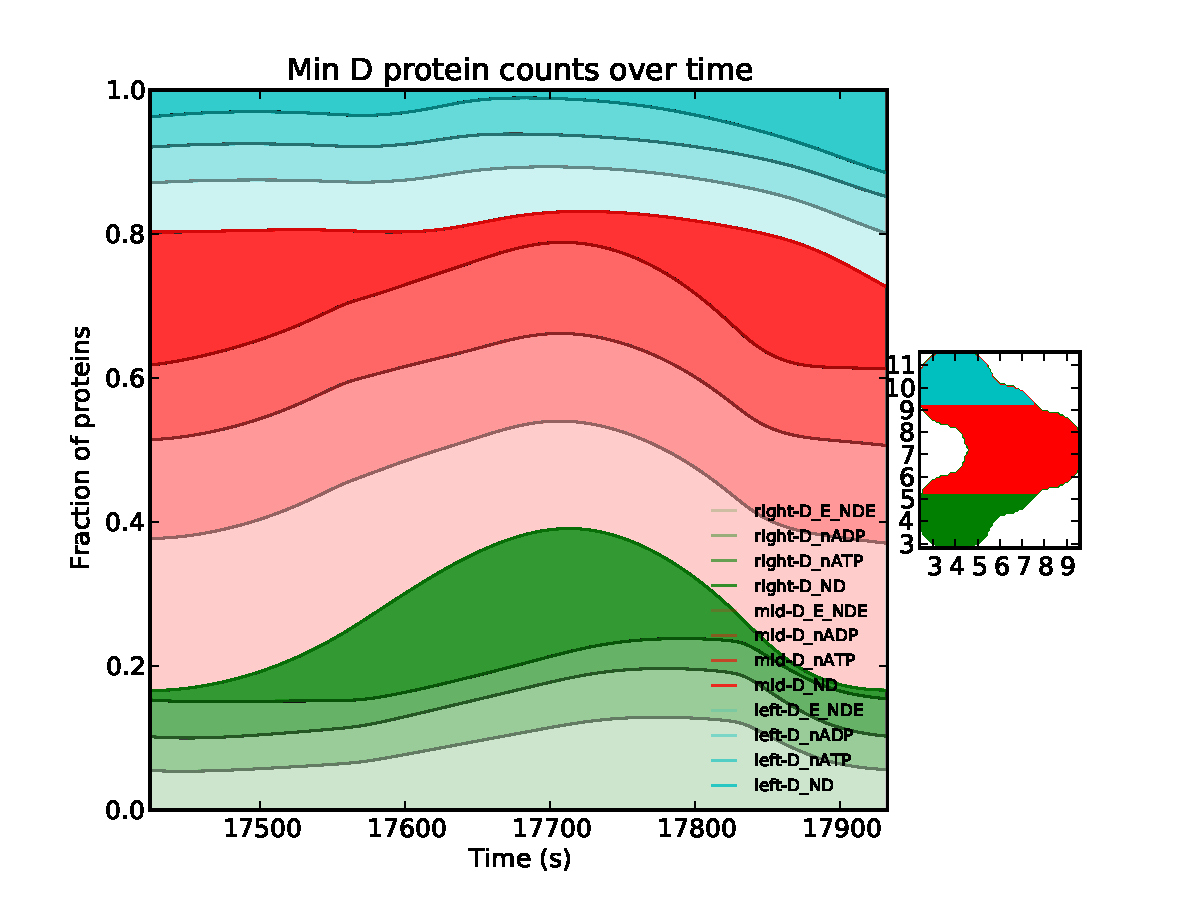
\includegraphics[width=\columnwidth]{../data/shape-randst/plots/box-plot_D--randst-25-600-600-9900-1500}
  %%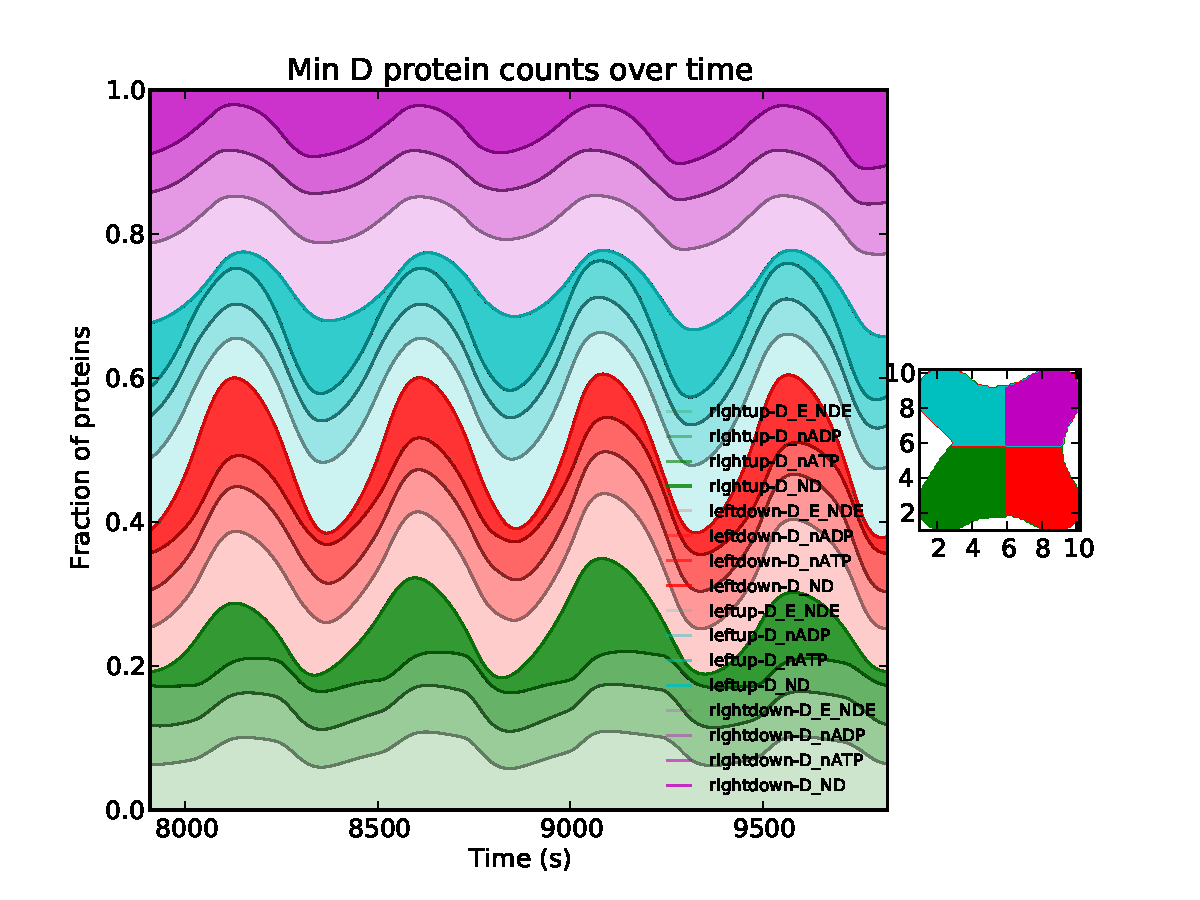
\includegraphics[width=\columnwidth]{../data/shape-randst/plots/box-plot_D--randst-25-600-600-9600-1500}arrow-plot-NflD-randst-25-600-800-9800-1500.pdf

  \caption{Total protein fluctuation in the A shaped shape.  The vertical axis shows stacked the total number
    of proteins that are of four different compound stages and in the
    different sections of the cell.}
  \label{total-oscillation-randst-96-plot}
\end{figure}



Our animations for this cell shape show a very interesting pattern.
The maxima oscillates from the right corner to the top corner, then
\emph{back to the right corner} then to the top corner again, then to
the left corner, then back to the top, then to the left, then to the
top again, then back to the right side.

\fixme{running larger and smaller.  Guessing the larger will do pole
  and pole, so talk about in terms of you have huge, pole and pole,
  then once get small enough double oscillations develop.  Why do they
  do that?  And hen you can do image plot for the one with consistent
  double oscillations.  Can right now explain reason for double
  oscillations.  Look at todo.txt.  The slightly varied guassian shape,
  so a little assymetric, doesn't change double oscillation pattern.}

Contour plot frames from the animations show the second maxima in the
lower left corner (immediately following the one in the upper middle
corner) will reside for a bit longer than the left corner maxima
preceding it.  These longer residing maxima will then be followed by a
switch, to the right corner, with a short, less intensive maxima
traveling through the center.  The MinE shows the same pattern. The
MinE that was just concentrated on the left corner during the first
maxima, after releasing the MinD from the membrane there, diffuses up
and attaches to the MinD on the upper corner membrane and begins to
release it.  During this process the MinE starts at the edges and
moves in towards the center of the maxima.  The center of the cup is a
little further away so it attaches to these outer ridges first and
then moves in.  After it eats at the corners and starts moving in the
MinD eventually travels back to set up a maxima in the left corner.
Watching the cytoplasmic MinE, something very interesting: It as well
maximizes twice in the left corner, but during the MinD's first maxima
in the left corner, the MinD has a maxima in the upper corner, and
during the MinD's second left maxima, the MinE travels to the right
corner and has a maxima there.  At the same time (during the second
MinD left corner maxima), there is a large amount of cytoplasmic
MinD:ATP on the right side.  The MinE does this becuase during the
first MinD left corner maxima, the MinE has just come off a maxima in
the right corner.  So it diffuses up to the upper corner and sets up
there.  During the second MinD left corner maxima, the MinE has just
come off the upper corner maxima.  It will diffuse into the right
corner and left corner.  In the left corner it interacts with the MinD
bound to the membrane there.  In the right corner it sits and
eventually diffuses away, but at a somewhat slow pace.  \fixme{An idea
  is that once the MinD travels back from the left corner after its
  second maxima there, it is not able tot set up a maxima in the upper
  corner as easily, since there is left over MinE there, which has
  just traveled from the right corner.  The problem with this is that
  the MinE doesn't seem to be maximized in the upper corner when the
  MinD is traveling back up from the left.}  The other idea is simply
that because the minE is traveling all the way from the right corner,
the longer time it takes to get there simply means that it all
concentrates on the left, leaving the upp and right side completely
open for the build up of MinD.  \fixme{Still dont quite get it but
  take a look at the other simulations and come back.} Actually, you
can see this effect very slightly watching the 98 shape, between the
center cap and the right corner.

Simulations of this shape that has the same height and dimensions .6
times the size (cells roughly $1.6\mu m$ from top to bottom) do not
exhibit the same pattern.  In these the MinD maxima oscillate quickly
back and forth between the two lower corner poles.

Simulations in which the two planar dimensions are 2 and then 3 times
the size (cells roughly $6\micron$ and $9\micron$, respectively, from top
to bottom) show no stable regular periodic pattern \fixme{although
  they haven't really run long enough to exhibit much.  They certainly
  won't show the double oscillation pattern, however.}  The animations
of $6\micron$ cells show that the MinD acts as a sort of traveling
cluster that is constantly being eaten away be MinE behind it.  When
this cluster enters a region of high curvature that ends in a dead end
corner it performs the polar maxima behavoir seen in the other
simulations, regrouping out away from the corner where it travels in
the opposite direction while being ``chased'' away by the MinE that
has itself maximized in the corner.  If it has just maximized in the
top corner, it regroups traveling downward and then naturally splits
into two groups that travel out and form maxima in the two opposite
bottom corners.  After maximizing in these two corners the two groups
recombine again in the center and travel in some direction together as
one cluster.  Simulations of the $9\micron$ cells show a similar roaming
cluster.  Although here, the maxima occur on non-polar walls often,
and will often split into two roaming clusters that interact less
quickly and are less correlated than those seen in the $6\micron$ cell.

It seems that there is an approximate critical cell size for which the
MinD will act in these ``wandering cluster'' formations.  The cell is
large enough so that there is a loss of MinD correlation between the
opposite sides (the protein in the right corner at any time is too far
away from the left to immediately affect the protein there).



%% \begin{center}
%%   \begin{figure}
%%     {\includegraphics[width=\paperwidth]{../data/shape-randst/plots/image-plot_E--randst-25-602-602-9900-1500}}
%%     \caption{Attempt at adding image plot to paper.}
%%     \label{image-plot}
%%   \end{figure}
%% \end{center}


\subsubsection{Randst-97-}
\begin{figure}
  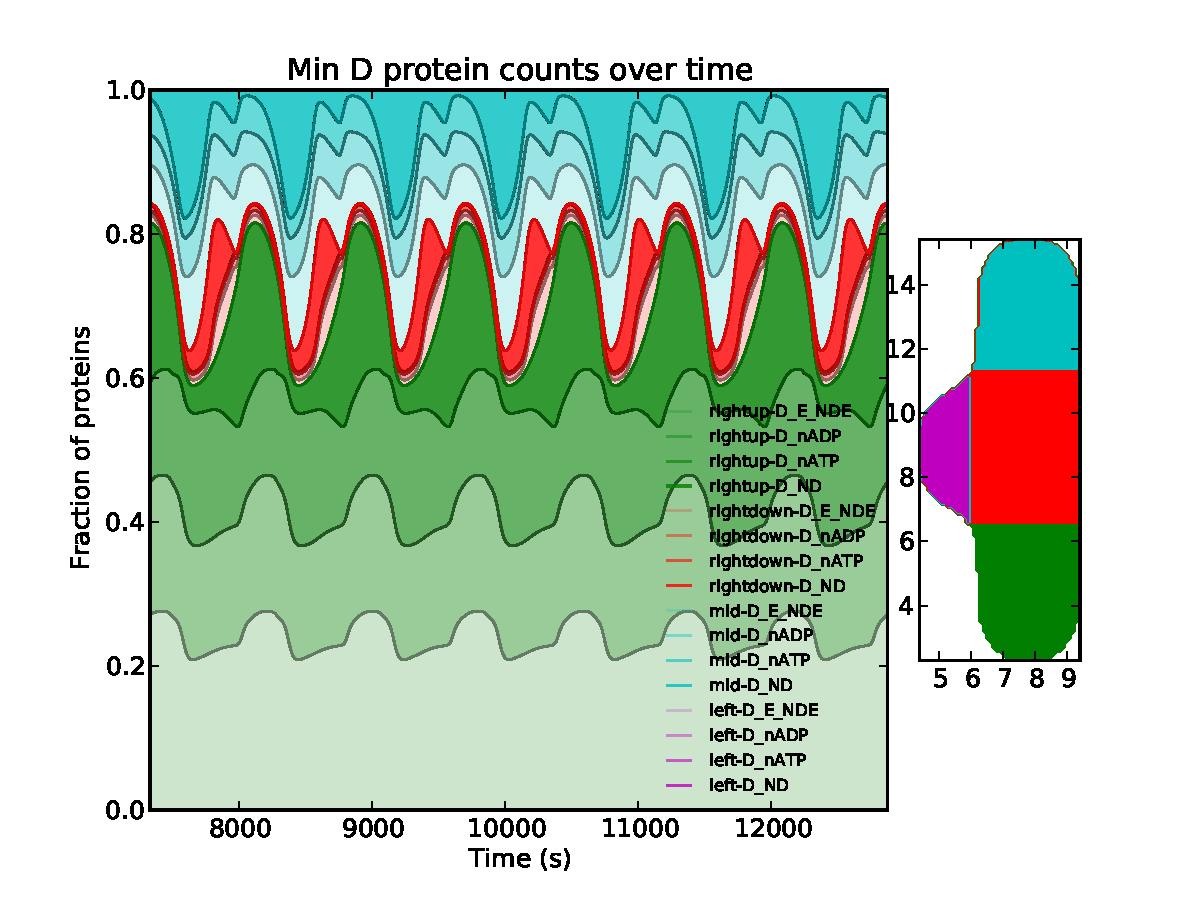
\includegraphics[width=\columnwidth]{../data/shape-randst/plots/box-plot_D--randst-25-800-600-9700-1500}
  %%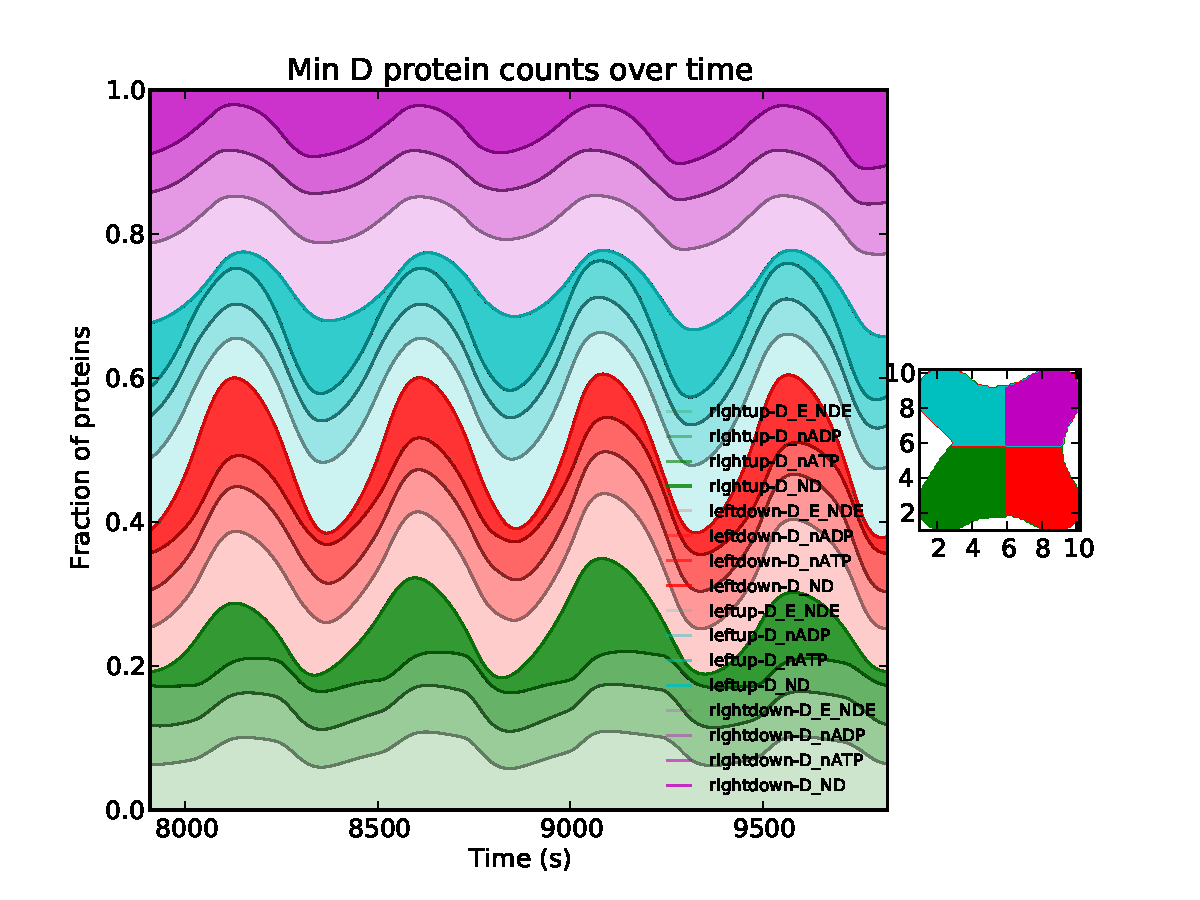
\includegraphics[width=\columnwidth]{../data/shape-randst/plots/box-plot_D--randst-25-600-600-9600-1500}
  \caption{Total protein fluctuation in the sideways flying saucer
    pancake cell shape.  The vertical axis shows stacked the total
    number of proteins that are of four different compound stages and
    in the different sections of the cell.}
  \label{box-97}
\end{figure}

Early on in its simulation the sideways flying saucer pancake shape
shows a clear breakdown of an unstable equilibrium oscillation.  We
have set the intial conditions so that MinD density is highly
concentrated to the left of a dividing line that runs parrallel to the
left vertical side.  For the first number of oscillations the maxima
trade off right to left, from a high peak in the rightward middle
compartment to vertically opposed peaks in the poles of the long axis
of the cell.  This is seen in the first part of Figure~\ref{box-97},
where the lower and upper sections peak in unison, and the middle
right section peaks $\pi$ radians removed from these.  After a few
oscillations the back and forth oscillations tip toward the vertical
direction and the system loses its initial oscillation pattern.  It
falls quickly instead into a back and forth pattern between the two
opposing endcaps.  The oscillation at this point is reminiscent of the
pills shape oscillation, once again showing the robust nature of the
back and forth, two pole pattern.

During each period, directly after one of the polar maxima has
subsided, there is a small spike with the regular maxima pattern (a
spike in membrane bound MinD:ATP immediately followed by a spike in
membrane bound MinD:MinE:ATP) seen in the small middle right
compartment section.  The animations show that the MinD, oscillating
back and forth between the upper and lower poles, seems to catch and
lag in the indentation for a bit before moving on.  Once again the
positive radius of curvature acts as an attractive place for MinD to
cluster on the walls, and it is not released to move on through the
cytoplasm again until MinE has formed its ring and completely reacted
it away.


\subsubsection{Randst-96-Star}
\begin{figure}
  \includegraphics[width=\columnwidth]{../data/shape-randst/plots/box-plot_D--randst-25-700-700-9600-1500}
  %%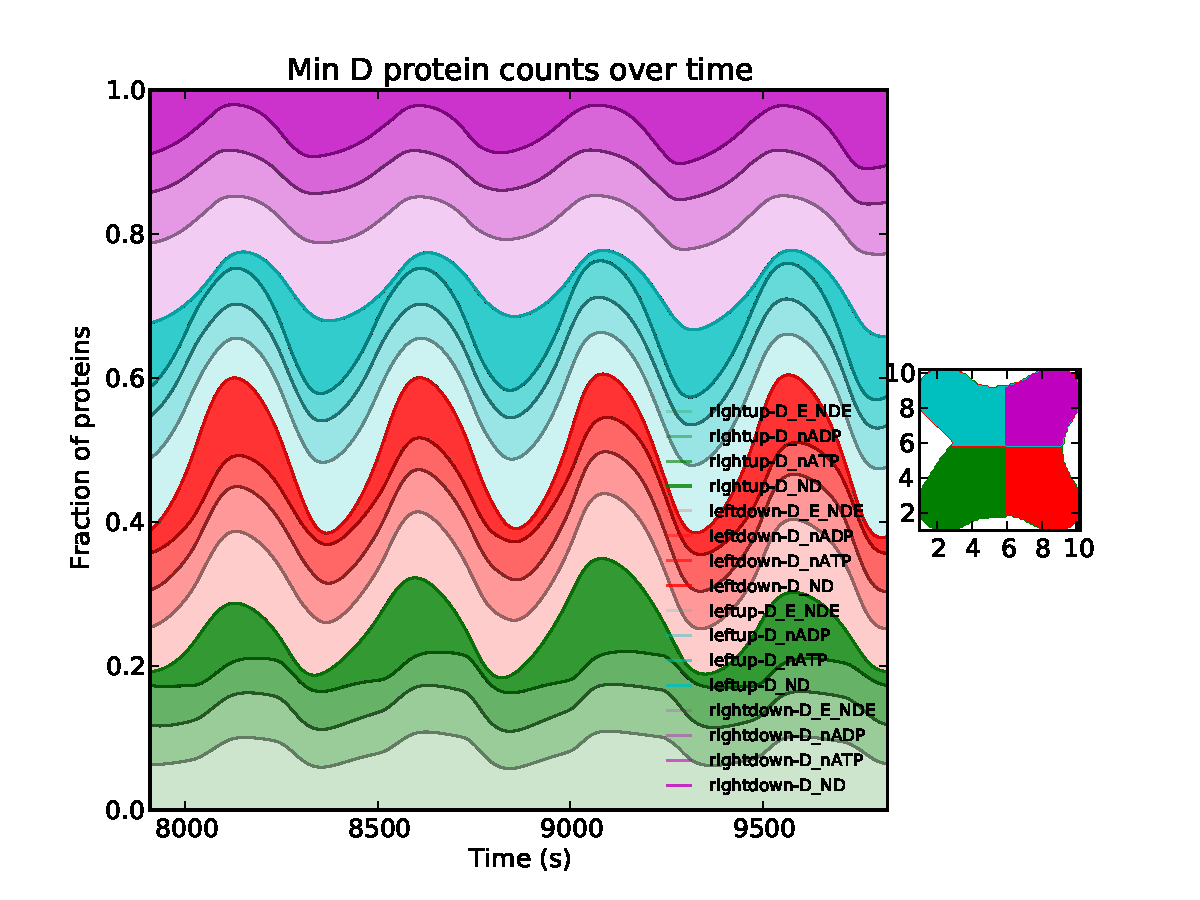
\includegraphics[width=\columnwidth]{../data/shape-randst/plots/box-plot_D--randst-25-600-600-9600-1500}
  \caption{Total protein fluctuation in the star cell shape.  The vertical axis shows stacked the total
    number of proteins that are of four different compound stages and
    in the different sections of the cell.}
  \label{box-96}
\end{figure}

This clover shape finds a regular oscillatory behavoir after about
seven periods that consists of two maxima that peak regularly in the
corners accross from each other at the same times (Figure
\ref{box-96}) and then again opposing maxima that peak at the same
time in the other two corners.\fixme{should try some different
  starting conditions with this to see if there's another patter.}

Looking at at few periods in detail.  We find that there is a small
increase in cytoplasmic MinE always directly before the the beggining
of climb in the membrane bound MinE peak.  Also, there is at any one
time a very large amount more of minE that is membrane bound then
cytoplasmic in any ones section.  A difference of a factor of roughly
20 when membrane MinE is at its peak, and roughly 12 when membrane
MinE is at it's minimum.  There seem to be two modes of oscillation,
each exhibiting a density peak maxima that moves back and forth
diagonaly from one corner to the opposite, as if there were two
overlapping, criss-crossed cells oscillating.  In the box plot this is
seen as roughly coinciding membrane minD peaks in the lower left and
right corners, followed one pi later in peaks in the upper right and
upper left corners.  Interesting that this did not exhibit
counterclockwise motion that Huangs 2008 paper might suggest.  Should
run sims that start in the wacky way that just started running with
triangles.
\newline


We haven't simulated long enough yet, so no real pattern has shown
itself.  There's certainly oscillations, and it's almost as if there's
competing modes - top to bottom, left to right, corner to corner, etc.
Interesting.

\fixme{maybe?}The animations seem to relax into a pattern in which the oscillations
go from the smallest corner, out to the other three, and then back to
the smallest corner?  \fixme{There isn't enough data to see properly
  though, need to run for longer.}


\section{Interpretation of Data}
\section{Conclusion}
\section*{Appendix}
\bibliography{paper}






\section{Below are NOTES for the Writing}

Figure \ref{total-oscillation-triangle-plot} shows the equivalent
motion and transference between compound states for the triangular
states as Figure \ref{total-oscillation-plot} does for the pill shaped
cells.  The equilateral triangular shows that in all three sections
there is a spike in wall attached MinD-ATP directly followed by a
spike in wall attached MinD-MinE-ATP.  The pill had shown a similar
pattern except that the mid section exhibited no such pronounced
spike.  Interestingly, the right and mid sections show spikes at
similar times when compared to the left section spikes, which seem to
oscillate in a manner shifted pi off from the other two.  This
behavoir shows itself in the animations, which show a relaxation into
a stable oscillation from a maxima in one corner to a double maxima in
the other two corners, and back again.  The left section heights are
roughly twice that of the right section heights.  The simulations are
started with higher concentrations of proteins in primarily the right
section, with some overlap into the middle section, so that perhpas
this oscillation pattern seems reasonable.  However, it's interesting
to note that the oscillations, started with assymmetric density, do
not naturally rotate around the corners of the triangle in a circular
pattern.


It seems as well that there is a desired oscillation maxima for the
particular shape and size of the cell, as can be seen by the
relaxation, over the first four periods, to a regular maximal height
of the right and left sections' total protein at the height of each spike.

\fixme{Note to make sure I'm interpreting the iscosolese triangle data
  correctly: the triangle sides are 5,5,3, and the higher density
  starts in the corner that is opposite the short side.  This corner
  is covered by the right section.  I've verified this by looking at
  the protein\_microscopy and drawing a little picture, which is on my
  desk...if you dare look for something on my desk!!!}  The iscosolese
triangle starts its simulation with a higher concentration of protein
in the section that is opposite the shorter side.  It quickly relaxes
into a stable oscillation pattern.  This pattern shows that right
corner section regularly has higher spikes in total protein than the
other sections, and that its spikes appear one pi removed from the
spikes for the other two sections.  This a similar behavoir to that
which is seen in the equilateral triangle, differening in that it
converges more quickly towards this behavoir and that it shows a
greater exageration in the height of protein buildup in the right most
section.

\fixme{Note on interpretation of 3-4-5 triangle: the higher density
  starts to the right of a vertical line that is parrallel to the
  second longest side in the triangle (the longer of the two
  non-hypotonuse sides).  This means the higher concentration covers
  the right angle and also the smaller angle in the triangle} The
3-4-5 triangle exhibits behavoir that I need more data to properly
observe.  I does not converge as quickly as that for the iscosolese or
equilateral triangles.



\end{document}
